\documentclass[a4paper, 12pt]{report}
\usepackage[utf8]{inputenc}    
\usepackage[T1]{fontenc}
\usepackage[french]{babel}
\usepackage{hyperref}
\usepackage{setspace}
\usepackage{newtxtext,newtxmath}
\usepackage[top=3cm, bottom=3cm, left=3cm, right=3cm]{geometry}
\usepackage[explicit]{titlesec}
\usepackage{graphicx}
\usepackage[stable]{footmisc}
\usepackage{wrapfig}
\usepackage{multicol}
\usepackage{minitoc}
\usepackage{plantuml}
\usepackage{listings}

\titleformat{\chapter}[display]{}{}{0pt} {
  \parbox{\textwidth} {
    \textbf{\fontsize{30}{30}\selectfont\thechapter.\hspace{0.5cm}\LARGE#1}\\
    \rule{\textwidth}{0.4pt}
  }
}
\titleformat{name=\chapter,numberless}[display]{}{}{0pt} {
  \parbox{\textwidth}{
    \LARGE\textbf{#1}\\
    \rule{\textwidth}{0.4pt}
  }
}

\hypersetup{
    colorlinks=true,
    urlcolor=black,
    linkcolor= black,
    citecolor=black
}

\mtcsetrules{*}{off}

\definecolor{backcolor}{rgb}{0.95,0.95,0.95}
\definecolor{numbers}{rgb}{0.5,0.5,0.5}
\lstdefinestyle{mystyle}{
    backgroundcolor=\color{backcolor},   
    aboveskip=3mm,
    belowskip=3mm,
    showstringspaces=false,
    columns=flexible,
    basicstyle={\small\ttfamily},
    numbers=none,
    breaklines=true,
    breakatwhitespace=true,
    tabsize=3,
    framexleftmargin=16pt,
    framextopmargin=6pt,
    framexbottommargin=6pt, 
    frame=tb, 
    framerule=0pt,
    numbers=left,
    numbersep=20pt,
    numberstyle=\tiny\color{numbers},
}
\lstset{style=mystyle}

\begin{document}
\renewcommand \partname{\thispagestyle{empty}}
\doparttoc

\thispagestyle{empty}
\begin{center}  
\begin{multicols}{2}
  \flushleft
  \null
  
\includegraphics[width=\columnwidth]{../res/logo-iut.png}
  \flushright
  \null
  \vspace{0.3cm}
  \large{Promotion 2020-2021}
\end{multicols}
\vspace{2cm}
\LARGE{\textit{Mise en place de traitements de masse relatifs à la relève des compteurs communiquants}}\\
\vspace{2cm}
\large{\textbf{Mémoire présenté en septembre 2021 par}}\\
\vspace{0.5cm}
\Large{\textit{Loïc STEINMETZ}}\\
\vspace{2cm}
\large{\textbf{En vue de l'obtention de la Licence Professionnelle}}\\
\vspace{0.5cm}
\fbox{
  \begin{minipage}{12cm}
    \begin{center}
      \null
      \vspace{0.3cm}
      \textbf{Métiers de l'Informatique}\\
      Conception, développement et test de logiciels\\
      Parcours Métiers du Génie Logiciel\\
      \null
    \end{center}
  \end{minipage}
}
\vspace{2.8cm}
\begin{multicols}{2}
  \flushleft
  \null
  \textbf{Alternance effectuée à :}\\
  Efluid\\
  2 bis, rue Ardant du Picq\\
  CS 10100 57004 METZ Cedex 01\\
  \flushright
  \null
  
\includegraphics[width=.6\columnwidth]{../res/logo-efluid.jpg}
\end{multicols}
\end{center}

\clearpage
\thispagestyle{empty}
\null
\clearpage

\thispagestyle{empty}
\begin{center}  
\begin{multicols}{2}
  \flushleft
  \null
  
\includegraphics[width=\columnwidth]{../res/logo-iut.png}
  \flushright
  \null
  \vspace{0.3cm}
  \large{Promotion 2020-2021}
\end{multicols}
\vspace{2cm}
\LARGE{\textit{Mise en place de traitements de masse relatifs à la relève des compteurs communiquants}}\\
\vspace{2cm}
\large{\textbf{Mémoire présenté en septembre 2021 par}}\\
\vspace{0.5cm}
\Large{\textit{Loïc STEINMETZ}}\\
\vspace{2cm}
\large{\textbf{En vue de l'obtention de la Licence Professionnelle}}\\
\vspace{0.5cm}
\fbox{
  \begin{minipage}{12cm}
    \begin{center}
      \null
      \vspace{0.3cm}
      \textbf{Métiers de l'Informatique}\\
      Conception, développement et test de logiciels\\
      Parcours Métiers du Génie Logiciel\\
      \null
    \end{center}
  \end{minipage}
}
\vspace{2.8cm}
\begin{multicols}{2}
  \flushleft
  \null
  \textbf{Alternance effectuée à :}\\
  Efluid\\
  2 bis, rue Ardant du Picq\\
  CS 10100 57004 METZ Cedex 01\\
  \flushright
  \null
  
\includegraphics[width=.6\columnwidth]{../res/logo-efluid.jpg}
\end{multicols}
\end{center}

\chapter*{Remerciements}
\addcontentsline{toc}{chapter}{Remerciements}
\thispagestyle{empty}

Je remercie tout particulièrement mon maître de stage, Alexandre L'HUILLIER, pour m'avoir fait bénéficier de ses compétences tout au long de mon année d'alternance. Merci à lui pour son professionalisme, sa confiance et sa disponibilité.\\

Je remercie également Jean-Luc THIRY, chef de service et Didier GRZEJSZCZAK, chef de filière, pour leur accompagnement général et pour ma bonne intégration au sein de l'entreprise.\\

Mes remerciements vont enfin à l'ensemble des membres du service auquel j'ai été intégré et que je n'ai pas encore cités : Patrice FRANTZ, Julien KEMPF, Fabienne MAMET, François MOLIN, Roderick PIERRE, Stéphane POIROT et Stéphane ROEDEL.

\part{Mémoire}
\renewcommand{\clearpage}{}
\chapter*{Sommaire}
\renewcommand\ptctitle{}
\parttoc
\thispagestyle{empty}
\renewcommand{\clearpage}{\newpage}
\clearpage

\chapter*{Abstract}
\addcontentsline{toc}{chapter}{Abstract}

Lorem ipsum dolor sit amet, consectetur adipiscing elit, sed do eiusmod tempor incididunt ut labore et dolore magna aliqua. Ut enim ad minim veniam, quis nostrud exercitation ullamco laboris nisi ut aliquip ex ea commodo consequat. Duis aute irure dolor in reprehenderit in voluptate velit esse cillum dolore eu fugiat nulla pariatur. Excepteur sint occaecat cupidatat non proident, sunt in culpa qui officia deserunt mollit anim id est laborum.

\chapter*{Introduction}
\addcontentsline{toc}{chapter}{Introduction}

Lorem ipsum dolor sit amet, consectetur adipiscing elit, sed do eiusmod tempor incididunt ut labore et dolore magna aliqua. Ut enim ad minim veniam, quis nostrud exercitation ullamco laboris nisi ut aliquip ex ea commodo consequat. Duis aute irure dolor in reprehenderit in voluptate velit esse cillum dolore eu fugiat nulla pariatur. Excepteur sint occaecat cupidatat non proident, sunt in culpa qui officia deserunt mollit anim id est laborum.

\chapter{Présentation de l'entreprise}

Lorem ipsum dolor sit amet, consectetur adipiscing elit, sed do eiusmod tempor incididunt ut labore et dolore magna aliqua. Ut enim ad minim veniam, quis nostrud exercitation ullamco laboris nisi ut aliquip ex ea commodo consequat. Duis aute irure dolor in reprehenderit in voluptate velit esse cillum dolore eu fugiat nulla pariatur. Excepteur sint occaecat cupidatat non proident, sunt in culpa qui officia deserunt mollit anim id est laborum.

\begin{figure}
  \begin{center}
    \begin{minipage}{4cm}
      \begin{center}
        
\includegraphics[height=2cm]{../res/logo-efluid.jpg}
        \caption{Efluid}
      \end{center}
    \end{minipage}
    \rule{1cm}{0cm}
    \begin{minipage}{4cm}
      \begin{center}
        
\includegraphics[height=2cm]{../res/logo-uem.jpg}
        \caption{UEM}
      \end{center}
    \end{minipage}
    \rule{1cm}{0cm}
    \begin{minipage}{4cm}
      \begin{center}
        
\includegraphics[height=2cm]{../res/logo-enedis.jpg}
        \caption{Enedis}
      \end{center}
    \end{minipage}
  \end{center}
\end{figure}

\chapter{Sujets traités}

\section{Généralités}

Lorem ipsum dolor sit amet, consectetur adipiscing elit, sed do eiusmod tempor incididunt ut labore et dolore magna aliqua. Ut enim ad minim veniam, quis nostrud exercitation ullamco laboris nisi ut aliquip ex ea commodo consequat. Duis aute irure dolor in reprehenderit in voluptate velit esse cillum dolore eu fugiat nulla pariatur. Excepteur sint occaecat cupidatat non proident, sunt in culpa qui officia deserunt mollit anim id est laborum.

\subsection{Environnement de développement}

Lorem ipsum dolor sit amet, consectetur adipiscing elit, sed do eiusmod tempor incididunt ut labore et dolore magna aliqua. Ut enim ad minim veniam, quis nostrud exercitation ullamco laboris nisi ut aliquip ex ea commodo consequat. Duis aute irure dolor in reprehenderit in voluptate velit esse cillum dolore eu fugiat nulla pariatur. Excepteur sint occaecat cupidatat non proident, sunt in culpa qui officia deserunt mollit anim id est laborum.

\begin{figure}
  \begin{center}
    \begin{minipage}{4cm}
      \begin{center}
        
\includegraphics[height=2cm]{../res/java.jpg}
        \caption{Java}
      \end{center}
    \end{minipage}
    \rule{1cm}{0cm}
    \begin{minipage}{4cm}
      \begin{center}
        
\includegraphics[height=2cm]{../res/oracle.png}
        \caption{Oracle}
      \end{center}
    \end{minipage}
    \rule{1cm}{0cm}
    \begin{minipage}{4cm}
      \begin{center}
        
\includegraphics[height=2cm]{../res/intellij.jpg}
        \caption{Intellij}
      \end{center}
    \end{minipage}
  \end{center}
\end{figure}

\subsection{Processus de production}

Lorem ipsum dolor sit amet, consectetur adipiscing elit, sed do eiusmod tempor incididunt ut labore et dolore magna aliqua. Ut enim ad minim veniam, quis nostrud exercitation ullamco laboris nisi ut aliquip ex ea commodo consequat. Duis aute irure dolor in reprehenderit in voluptate velit esse cillum dolore eu fugiat nulla pariatur. Excepteur sint occaecat cupidatat non proident, sunt in culpa qui officia deserunt mollit anim id est laborum.

\section{Développements courants}

Lorem ipsum dolor sit amet, consectetur adipiscing elit, sed do eiusmod tempor incididunt ut labore et dolore magna aliqua. Ut enim ad minim veniam, quis nostrud exercitation ullamco laboris nisi ut aliquip ex ea commodo consequat. Duis aute irure dolor in reprehenderit in voluptate velit esse cillum dolore eu fugiat nulla pariatur. Excepteur sint occaecat cupidatat non proident, sunt in culpa qui officia deserunt mollit anim id est laborum.

\section{Projet principal}

Lorem ipsum dolor sit amet, consectetur adipiscing elit, sed do eiusmod tempor incididunt ut labore et dolore magna aliqua. Ut enim ad minim veniam, quis nostrud exercitation ullamco laboris nisi ut aliquip ex ea commodo consequat. Duis aute irure dolor in reprehenderit in voluptate velit esse cillum dolore eu fugiat nulla pariatur. Excepteur sint occaecat cupidatat non proident, sunt in culpa qui officia deserunt mollit anim id est laborum.

\chapter{Traitement du projet industriel}

\section{Analyses préliminaires}

Lorem ipsum dolor sit amet, consectetur adipiscing elit, sed do eiusmod tempor incididunt ut labore et dolore magna aliqua. Ut enim ad minim veniam, quis nostrud exercitation ullamco laboris nisi ut aliquip ex ea commodo consequat. Duis aute irure dolor in reprehenderit in voluptate velit esse cillum dolore eu fugiat nulla pariatur. Excepteur sint occaecat cupidatat non proident, sunt in culpa qui officia deserunt mollit anim id est laborum.

\subsection{Analyse volumétrique}

Lorem ipsum dolor sit amet, consectetur adipiscing elit, sed do eiusmod tempor incididunt ut labore et dolore magna aliqua. Ut enim ad minim veniam, quis nostrud exercitation ullamco laboris nisi ut aliquip ex ea commodo consequat. Duis aute irure dolor in reprehenderit in voluptate velit esse cillum dolore eu fugiat nulla pariatur. Excepteur sint occaecat cupidatat non proident, sunt in culpa qui officia deserunt mollit anim id est laborum.

\subsection{Analyse des contextes de demande de publication de la relève}

Lorem ipsum dolor sit amet, consectetur adipiscing elit, sed do eiusmod tempor incididunt ut labore et dolore magna aliqua. Ut enim ad minim veniam, quis nostrud exercitation ullamco laboris nisi ut aliquip ex ea commodo consequat. Duis aute irure dolor in reprehenderit in voluptate velit esse cillum dolore eu fugiat nulla pariatur. Excepteur sint occaecat cupidatat non proident, sunt in culpa qui officia deserunt mollit anim id est laborum.

\subsection{Formation batch}

Lorem ipsum dolor sit amet, consectetur adipiscing elit, sed do eiusmod tempor incididunt ut labore et dolore magna aliqua. Ut enim ad minim veniam, quis nostrud exercitation ullamco laboris nisi ut aliquip ex ea commodo consequat. Duis aute irure dolor in reprehenderit in voluptate velit esse cillum dolore eu fugiat nulla pariatur. Excepteur sint occaecat cupidatat non proident, sunt in culpa qui officia deserunt mollit anim id est laborum.

\subsection{Formalisation du périmètre fonctionnel du projet}

Lorem ipsum dolor sit amet, consectetur adipiscing elit, sed do eiusmod tempor incididunt ut labore et dolore magna aliqua. Ut enim ad minim veniam, quis nostrud exercitation ullamco laboris nisi ut aliquip ex ea commodo consequat. Duis aute irure dolor in reprehenderit in voluptate velit esse cillum dolore eu fugiat nulla pariatur. Excepteur sint occaecat cupidatat non proident, sunt in culpa qui officia deserunt mollit anim id est laborum.

\begin{figure}[b]
  \begin{center}
    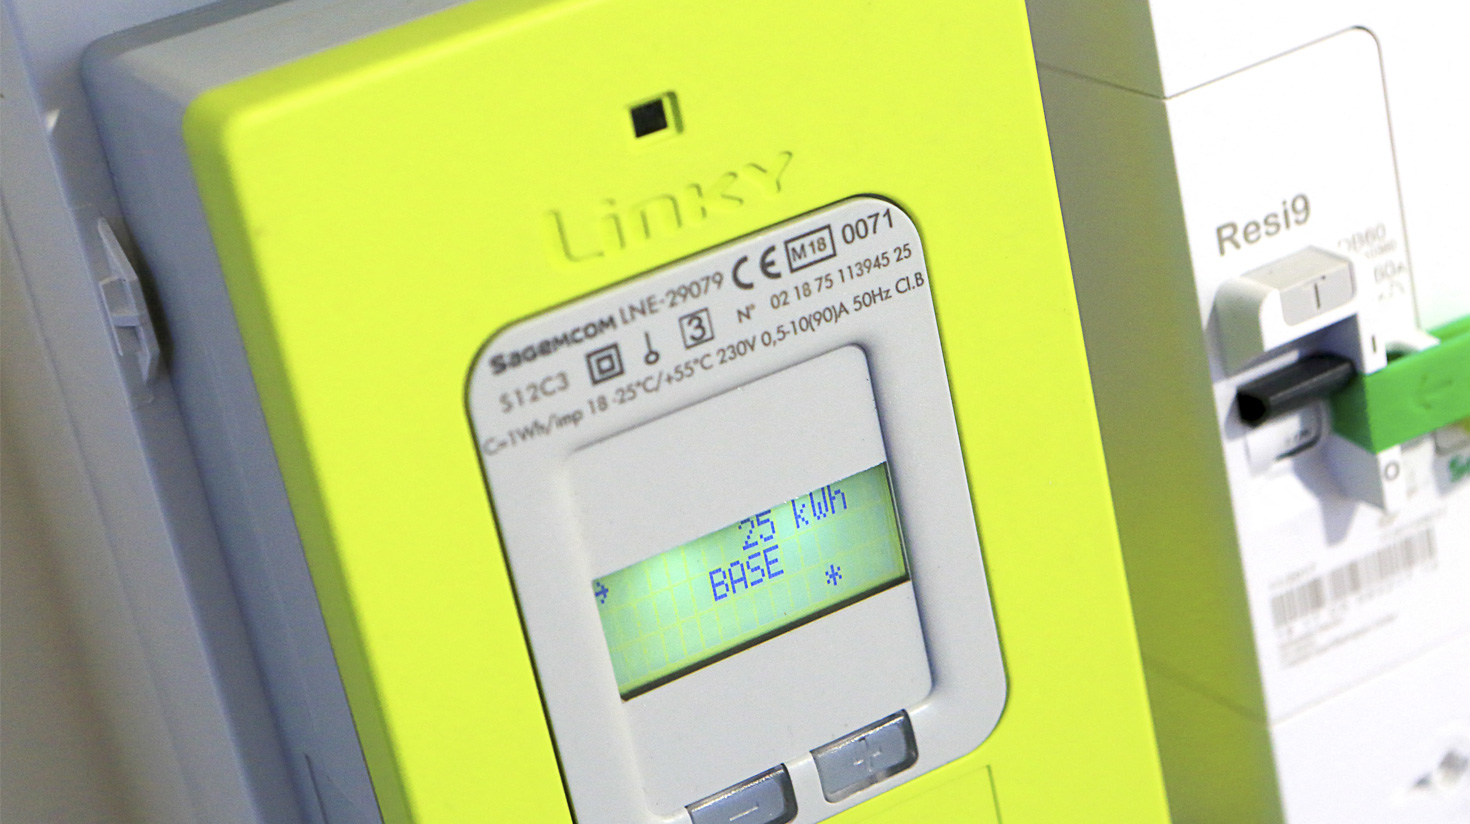
\includegraphics[height=4cm]{../res/linky.jpg}
    \caption{Compteur \textit{Linky}}
  \end{center}
\end{figure}

\section{Formalisation du besoin et planification}

Lorem ipsum dolor sit amet, consectetur adipiscing elit, sed do eiusmod tempor incididunt ut labore et dolore magna aliqua. Ut enim ad minim veniam, quis nostrud exercitation ullamco laboris nisi ut aliquip ex ea commodo consequat. Duis aute irure dolor in reprehenderit in voluptate velit esse cillum dolore eu fugiat nulla pariatur. Excepteur sint occaecat cupidatat non proident, sunt in culpa qui officia deserunt mollit anim id est laborum.

\subsection{Description fonctionnelle du batch}

Lorem ipsum dolor sit amet, consectetur adipiscing elit, sed do eiusmod tempor incididunt ut labore et dolore magna aliqua. Ut enim ad minim veniam, quis nostrud exercitation ullamco laboris nisi ut aliquip ex ea commodo consequat. Duis aute irure dolor in reprehenderit in voluptate velit esse cillum dolore eu fugiat nulla pariatur. Excepteur sint occaecat cupidatat non proident, sunt in culpa qui officia deserunt mollit anim id est laborum.

\subsection{Découpage technique}

Lorem ipsum dolor sit amet, consectetur adipiscing elit, sed do eiusmod tempor incididunt ut labore et dolore magna aliqua. Ut enim ad minim veniam, quis nostrud exercitation ullamco laboris nisi ut aliquip ex ea commodo consequat. Duis aute irure dolor in reprehenderit in voluptate velit esse cillum dolore eu fugiat nulla pariatur. Excepteur sint occaecat cupidatat non proident, sunt in culpa qui officia deserunt mollit anim id est laborum.

\section{Conception et implémentation}

Lorem ipsum dolor sit amet, consectetur adipiscing elit, sed do eiusmod tempor incididunt ut labore et dolore magna aliqua. Ut enim ad minim veniam, quis nostrud exercitation ullamco laboris nisi ut aliquip ex ea commodo consequat. Duis aute irure dolor in reprehenderit in voluptate velit esse cillum dolore eu fugiat nulla pariatur. Excepteur sint occaecat cupidatat non proident, sunt in culpa qui officia deserunt mollit anim id est laborum.

\subsection{Solutions d'intégration du batch}

Lorem ipsum dolor sit amet, consectetur adipiscing elit, sed do eiusmod tempor incididunt ut labore et dolore magna aliqua. Ut enim ad minim veniam, quis nostrud exercitation ullamco laboris nisi ut aliquip ex ea commodo consequat. Duis aute irure dolor in reprehenderit in voluptate velit esse cillum dolore eu fugiat nulla pariatur. Excepteur sint occaecat cupidatat non proident, sunt in culpa qui officia deserunt mollit anim id est laborum.

\subsection{Architecture générale}

Lorem ipsum dolor sit amet, consectetur adipiscing elit, sed do eiusmod tempor incididunt ut labore et dolore magna aliqua. Ut enim ad minim veniam, quis nostrud exercitation ullamco laboris nisi ut aliquip ex ea commodo consequat. Duis aute irure dolor in reprehenderit in voluptate velit esse cillum dolore eu fugiat nulla pariatur. Excepteur sint occaecat cupidatat non proident, sunt in culpa qui officia deserunt mollit anim id est laborum.

\subsection{Chargement des objets métiers}

Lorem ipsum dolor sit amet, consectetur adipiscing elit, sed do eiusmod tempor incididunt ut labore et dolore magna aliqua. Ut enim ad minim veniam, quis nostrud exercitation ullamco laboris nisi ut aliquip ex ea commodo consequat. Duis aute irure dolor in reprehenderit in voluptate velit esse cillum dolore eu fugiat nulla pariatur. Excepteur sint occaecat cupidatat non proident, sunt in culpa qui officia deserunt mollit anim id est laborum.

\subsection{Implémentation des traitements}

Lorem ipsum dolor sit amet, consectetur adipiscing elit, sed do eiusmod tempor incididunt ut labore et dolore magna aliqua. Ut enim ad minim veniam, quis nostrud exercitation ullamco laboris nisi ut aliquip ex ea commodo consequat. Duis aute irure dolor in reprehenderit in voluptate velit esse cillum dolore eu fugiat nulla pariatur. Excepteur sint occaecat cupidatat non proident, sunt in culpa qui officia deserunt mollit anim id est laborum.

\subsection{Tests}

Lorem ipsum dolor sit amet, consectetur adipiscing elit, sed do eiusmod tempor incididunt ut labore et dolore magna aliqua. Ut enim ad minim veniam, quis nostrud exercitation ullamco laboris nisi ut aliquip ex ea commodo consequat. Duis aute irure dolor in reprehenderit in voluptate velit esse cillum dolore eu fugiat nulla pariatur. Excepteur sint occaecat cupidatat non proident, sunt in culpa qui officia deserunt mollit anim id est laborum.

\chapter*{Conclusion}
\addcontentsline{toc}{chapter}{Conclusion}

Lorem ipsum dolor sit amet, consectetur adipiscing elit, sed do eiusmod tempor incididunt ut labore et dolore magna aliqua. Ut enim ad minim veniam, quis nostrud exercitation ullamco laboris nisi ut aliquip ex ea commodo consequat. Duis aute irure dolor in reprehenderit in voluptate velit esse cillum dolore eu fugiat nulla pariatur. Excepteur sint occaecat cupidatat non proident, sunt in culpa qui officia deserunt mollit anim id est laborum.

\part{Annexes}
\renewcommand{\clearpage}{}
\chapter*{Table des annexes}
\renewcommand\ptctitle{}
\parttoc
\thispagestyle{empty}
\renewcommand{\clearpage}{\newpage}
\appendix

\chapter{Efluid : répartition des parts}
\label{appendix:efluid-parts}

\begin{center}
  \begin{plantuml}
    @startmindmap
    
    <style>
      node {
          LineColor black
          BackgroundColor #FFF
          RoundCorner 0
      }
      arrow {
          LineColor #000
      }
      grey {
        BackgroundColor #BBB
      }
    </style>

      * Efluid
      **_ 60%
      *** UEM
      **_ 30%
      *** Enedis
      **_ 10%
      *** CDC

    @endmindmap
  \end{plantuml}
\end{center}

\vspace{1cm}
\noindent\textbf{UEM :} Usine d'Electricité de Metz\\
\noindent\textbf{CDC :} Caisse des Dépôts et Consignations

\chapter{Efluid : organisation des services}
\label{appendix:efluid-organisation}

\begin{center}
  \begin{plantuml}
    @startmindmap
    
    <style>
      node {
          LineColor black
          BackgroundColor #FFF
          RoundCorner 0
      }
      arrow {
          LineColor #000
      }
      grey {
        BackgroundColor #BBB
      }
    </style>

      * Direction
      ** Direction informatique
      *** Technologies
      *** Développement : CRM et Facturation
      *** Développement : Comptage et réseaux <<grey>>
      ** Direction commerciale
      *** Expertise fonctionnelle : CRM et Facturation
      *** Expertise fonctionnelle : Comptage et réseaux
      *** Coordination et clients
      *** Prestation et projets
      ** Ginko

    @endmindmap
  \end{plantuml}
\end{center}

\chapter{Efluid : logiciel}
\label{appendix:logiciel}

\begin{center}
  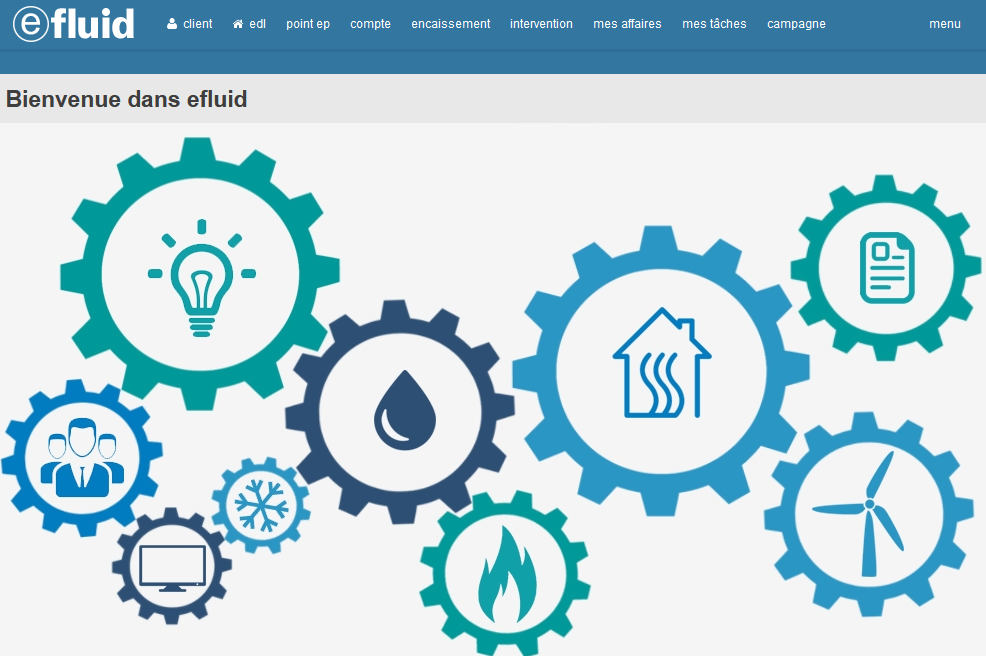
\includegraphics[height=8cm]{../res/efluid-1.png}
  \null
  \vspace{0.3cm}
  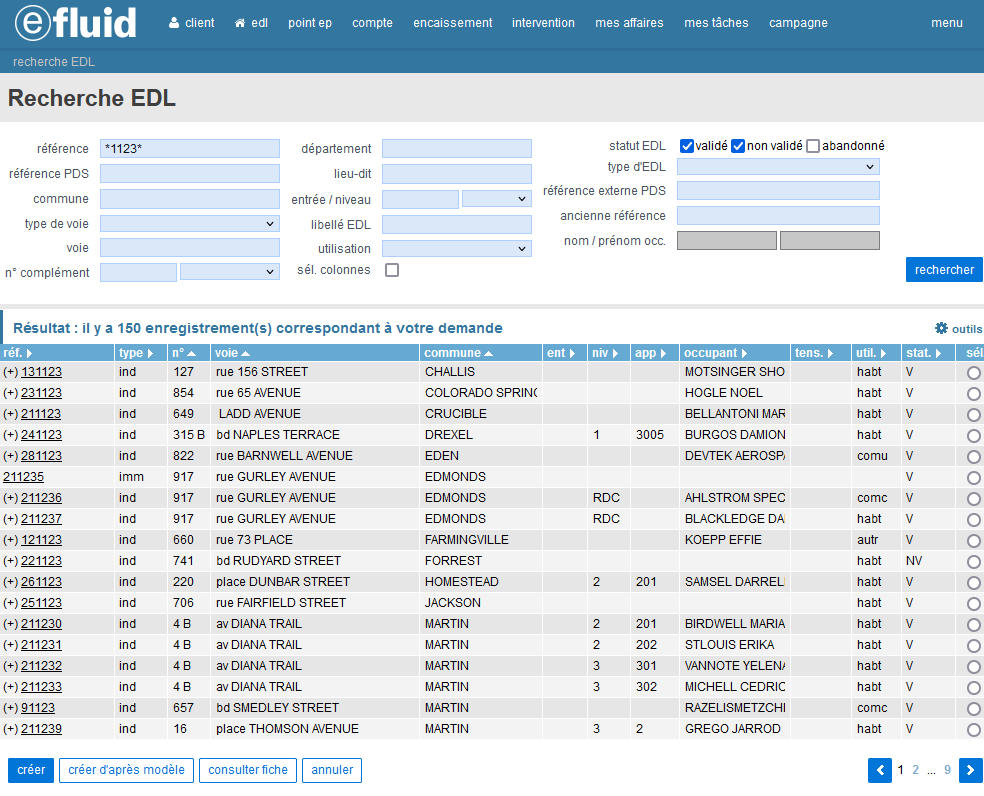
\includegraphics[height=9cm]{../res/efluid-2.png}
\end{center}

\chapter{Volumétrie}
\label{appendix:volumetrie}

\textit{Volumes estimés le 20/01/2021 à partir des copies des bases de données de production.}\\

Les données suivantes permettent d’évaluer le nombre de relèves concernées par le processus de demande de publication quel que soit leur contexte de création.\\

\begin{itemize}
  \item \textbf{UEM}
  \begin{itemize}
    \item \approx\space 3 500 relèves impliquant une création d'échange
    \item \approx\space 91 000 relèves créées
    \item Ratio demande de publication / création de relève : \approx\space 4\%
  \end{itemize}
  \item \textbf{Enedis IDF}
  \begin{itemize}
    \item \approx\space 6 300 000 relèves impliquant une création d'échange
    \item \approx\space 6 400 000 relèves créées
    \item Ratio demande de publication / création de relève : \approx\space 99\%
  \end{itemize}
  \item \textbf{Enedis Est}
  \begin{itemize}
    \item \approx\space 3 000 000 relèves impliquant une création d'échange
    \item \approx\space 3 100 000 relèves créées
    \item Ratio demande de publication / création de relève : \approx\space 95\%
  \end{itemize}
  \item \textbf{Enedis Ouest}
  \begin{itemize}
    \item \approx\space 5 200 000 relèves impliquant une création d'échange
    \item \approx\space 5 400 000 relèves créées
    \item Ratio demande de publication / création de relève : \approx\space 96\%
  \end{itemize}
  \item \textbf{Enedis Méditerranée}
  \begin{itemize}
    \item \approx\space 5 200 000 relèves impliquant une création d'échange
    \item \approx\space 5 400 000 relèves créées
    \item Ratio demande de publication / création de relève : \approx\space 96\%
  \end{itemize}
\end{itemize}
\vspace{0.6cm}

Les données suivantes permettent d’évaluer le nombre de relèves concernées par le processus de demande de publication en ne considérant que les relèves réalisées via un compteur \textit{\textit{Linky}}.\\

\begin{itemize}
  \item \textbf{Enedis IDF}
  \begin{itemize}
    \item \approx\space 5 400 000 relèves de compteurs \textit{\textit{Linky}} impliquant une création d'échange
    \item \approx\space 5 500 000 relèves de compteur \textit{\textit{Linky}} créées
    \item Ratio demande de publication / création de relève : \approx\space 98\%
    \item \approx\space 85\% des relèves créées concernent un compteur \textit{\textit{Linky}}
    \item \approx\space 85\% des demandes de publication de la relève concernent une relève de compteur \textit{\textit{Linky}}
  \end{itemize}
  \item \textbf{Enedis Est}
  \begin{itemize}
    \item \approx\space 2 500 000 relèves de compteurs \textit{Linky} impliquant une création d'échange
    \item \approx\space 2 600 000 relèves de compteur \textit{Linky} créées
    \item Ratio demande de publication / création de relève : \approx\space 95\%
    \item \approx\space 89\% des relèves créées concernent un compteur \textit{Linky}
    \item \approx\space 85\% des demandes de publication de la relève concernent une relève de compteur \textit{Linky}
  \end{itemize}
  \item \textbf{Enedis Ouest}
  \begin{itemize}
    \item \approx\space 4 600 000 relèves de compteurs \textit{Linky} impliquant une création d'échange
    \item \approx\space 4 800 000 relèves de compteur \textit{Linky} créées
    \item Ratio demande de publication / création de relève : \approx\space 96\%
    \item \approx\space 89\% des relèves créées concernent un compteur \textit{Linky}
    \item \approx\space 90\% des demandes de publication de la relève concernent une relève de compteur \textit{Linky}
  \end{itemize}
  \item \textbf{Enedis Méditerranée}
  \begin{itemize}
    \item \approx\space 4 800 000 relèves de compteurs \textit{Linky} impliquant une création d'échange
    \item \approx\space 4 900 000 relèves de compteur \textit{Linky} créées
    \item Ratio demande de publication / création de relève : \approx\space 97\%
    \item \approx\space 90\% des relèves créées concernent un compteur \textit{Linky}
    \item \approx\space 91\% des demandes de publication de la relève concernent une relève de compteur \textit{Linky}
  \end{itemize}
\end{itemize}

\chapter{Planification}
\label{appendix:planification}

\begin{itemize}
  \item \textbf{Planification annuelle :}\\
\end{itemize}

\begin{center}
  \begin{plantuml}
    @startuml

    skinparam monochrome true
    scale 1024 width
    scale 768 height

    printscale monthly zoom 1.4
    project starts the 2020-09-01

    [Pré-conception] starts 2020-09-01
    [Pré-conception] ends 2020-12-31
    [Conception] starts 2020-12-01
    [Conception] ends 2021-05-31
    [Développements] starts 2021-03-01
    [Développements] ends 2021-08-31

    @enduml
  \end{plantuml}
\end{center}
\vspace{1cm}

\begin{itemize}
  \item \textbf{Planification de l'implémentation :}\\
\end{itemize}

\begin{center}
  \begin{plantuml}
    @startuml

    skinparam monochrome true
    scale 1024 width
    scale 768 height

    printscale weekly
    project starts the 2021-02-01

    [Formalisation du besoin] starts 2021-02-01
    [Formalisation du besoin] ends 2021-02-15
    --
    [Intégration de la solution] starts 2021-02-08
    [Intégration de la solution] ends 2021-03-07
    --
    [Squelette batch] starts 2021-03-01
    [Squelette batch] ends 2021-03-15
    --
    [Implémentation des chargements] starts 2021-03-16
    [Implémentation des chargements] ends 2021-05-01
    --
    [Implémentation des process] starts 2021-04-16
    [Implémentation des process] ends 2021-06-01
    --
    [Tests] starts 2021-06-01
    [Tests] ends 2021-07-31

    [Squelette batch]->[Implémentation des chargements]
    [Implémentation des chargements]->[Tests]
    [Implémentation des process]->[Tests]
    [Intégration de la solution]->[Tests]

    @enduml
  \end{plantuml}
\end{center}

\chapter{Traitement de la demande de publication}
\label{appendix:process}

\begin{itemize}
  \item \textbf{Structure des traitements :}\\
\end{itemize}

\begin{center}
  \begin{plantuml}
    @startuml

    skinparam monochrome true
    left to right direction

    GestionDemandePublicationReleveProcess <|-- GestionDemandePublicationAvecDonneesProcess
    GestionDemandePublicationReleveProcess <|-- GestionDemandePublicationEstimationReleveFacturationProcess
    GestionDemandePublicationReleveProcess <|-- GestionDemandePublicationImportReleveAvecDonneesProcess

    @enduml
  \end{plantuml}
\end{center}
\vspace{0.5cm}

\begin{itemize}
  \item \textbf{Processus appelants :}\\
  \begin{itemize}
    \item Saisie d'une relève par un agent
    \item Auto-relève lors d'une demande de prestation
    \item CRI\footnote{Compte-Rendu d'Intervention} avec saisie d'une relève
    \item REL005MT : Batch de calcul des consommations
    \item REL019MT : Batch d'import des télérelèves gaz
    \item FAC002MT : Batch d'estimation des relèves pour EDP\footnote{Elément De Population} facturable
    \item FAC006MT : Batch de calcul des factures
    \item FAC020MT : Batch d'estimation des relèves pour EDP non factuable
    \item \underline{LKY06} : Interface de récupération des données \textit{Linky}
  \end{itemize}
\end{itemize}

\chapter{\textit{Design Pattern}\footnote{Patron de conception} : Stratégie}
\label{appendix:strategy}

\begin{itemize}
  \item \textbf{Sans stratégie :}\\
\end{itemize}

\begin{center}
  \begin{plantuml}
    @startuml

    skinparam monochrome true
    scale 250 height

    class Process {
      executer() : void
    }
    class SousProcess1 {
      executer1() : void
    }
    class SousProcess2 {
      executer2() : void
    }
    class SousProcess3 {
      executer3() : void
    }

    Process ..> SousProcess1
    Process ..> SousProcess2
    Process ..> SousProcess3

    @enduml
  \end{plantuml}
\end{center}
\vspace{0.5cm}

\begin{lstlisting}
public class Process {

    public void executer() {
        if (condition1) {
          new SousProcess1().exectuer1();
        } else if (condition2) {
          new SousProcess2().executer2();
        } else if (condition3) {
          new SousProcess3.executer3();
        }
    }    
}
\end{lstlisting}
\clearpage

\begin{itemize}
  \item \textbf{Avec stratégie :}\\
\end{itemize}

\begin{center}
  \begin{plantuml}
    @startuml

    skinparam monochrome true

    class Process {
      -service : Service
      +executer() : void
    }
    interface Service {
      +executerService() : void
    }
    class SousProcess1 {
      +executerService() : void
    }
    class SousProcess2 {
      +executerService() : void
    }
    class SousProcess3 {
      +executerService() : void
    }

    Process *-- Service
    Service <-- SousProcess1
    Service <-- SousProcess2
    Service <-- SousProcess3

    @enduml
  \end{plantuml}
\end{center}
\vspace{0.5cm}

\begin{lstlisting}
  public class Process {

      private Service service;

      public Process(Service service) {
        this.service = service;
      }
  
      public void executer() {
          service.executerService();
      }    
  }
  \end{lstlisting}

\chapter{Batch : architecture et implémentation}
\label{appendix:batch}

\begin{itemize}
  \item \textbf{Architecture :}\\
\end{itemize}

\begin{center}
  \begin{plantuml}
    @startuml

    scale 450 height
    skinparam monochrome true

    abstract class ProgramBatchDAO
    abstract class ProgramBatch
    class ParallelJobLauncher
    abstract class AbstractAppBatchJob
    abstract class BatchJobDAO

    ProgramBatch .u.> ProgramBatchDAO
    ProgramBatch .d.> ParallelJobLauncher
    ParallelJobLauncher .d.> AbstractAppBatchJob
    AbstractAppBatchJob .d.> BatchJobDAO

    @enduml
  \end{plantuml}
\end{center}
\clearpage

\begin{itemize}
  \item \textbf{Implémentation :}\\
\end{itemize}

\begin{center}
  \begin{plantuml}
    @startuml

    skinparam monochrome true
    scale 250 height

    class DemandePublicationRekeveProgramDAO
    class ERequeteDemandePublicationReleveBatchDAO
    class DemandePublicationReleveJobDAO

    DemandePublicationRekeveProgramDAO .d.> ERequeteDemandePublicationReleveBatchDAO
    DemandePublicationReleveJobDAO .u.> ERequeteDemandePublicationReleveBatchDAO

    @enduml
  \end{plantuml}
\end{center}
\begin{center}
  \begin{plantuml}
    @startuml

    skinparam monochrome true
    scale 150 height

    class DemandePublicationReleveProgram
    class DemandePublicationReleveBatchConstantes

    DemandePublicationReleveProgram .d.> DemandePublicationReleveBatchConstantes

    @enduml
  \end{plantuml}
\end{center}
\begin{center}
  \begin{plantuml}
    @startuml

    skinparam monochrome true
    left to right direction

    class DemandePublicationReleveJob
    class GestionDemandePublicationReleveProcess #BBB
    class ECountDemandePublicationReleveType
    class DemandePublicationReleveBatchDAOExceptions

    DemandePublicationReleveJob ..> GestionDemandePublicationReleveProcess
    DemandePublicationReleveJob ..> ECountDemandePublicationReleveType
    DemandePublicationReleveJob ..> DemandePublicationReleveBatchDAOExceptions

    @enduml
  \end{plantuml}
\end{center}

\tableofcontents
\thispagestyle{empty}

\chapter*{Résumé}
\thispagestyle{empty}

Lorem ipsum dolor sit amet, consectetur adipiscing elit, sed do eiusmod tempor incididunt ut labore et dolore magna aliqua. Ut enim ad minim veniam, quis nostrud exercitation ullamco laboris nisi ut aliquip ex ea commodo consequat. Duis aute irure dolor in reprehenderit in voluptate velit esse cillum dolore eu fugiat nulla pariatur. Excepteur sint occaecat cupidatat non proident, sunt in culpa qui officia deserunt mollit anim id est laborum.

\end{document}